% small.tex
\documentclass{beamer}
%\usetheme{default}
\usetheme{Warsaw}
\usecolortheme{whale}
\usepackage{tikz}
\usepackage[absolute,overlay]{textpos}
\usepackage{soul}
\usepackage{pdfpages}
\usepackage[most]{tcolorbox}
%\usepackage{multirow}
\usepackage{tikz,amsmath,array}
\usepackage{hyperref}

\newcommand{\greekbf}[1]{\boldsymbol{\mathrm{#1}}}
\newcommand{\btVFill}{\vskip0pt plus 1filll}
\newcolumntype{P}[1]{>{\centering\arraybackslash}p{#1}}

%\setbeamertemplate{background}[grid][step=.25\textwidth]

\title[Osteo Paradox]{Latent trait models and other Bayesian solutions to the Osteological Paradox}
%\subtitle
\author{Michael Holton Price}
\institute[SFI] {
	Santa Fe Institute\\
	MichaelHoltonPrice@gmail.com\\
	\line(1,0){0}\\
	Radiocarbon Universe Webinar Series\\
	09 Jun 2020\\
}
%\date{05 Feb 2014}
\date{}

% Note: default dimensions are 128 mm by 96 mm (4 x 3)
\begin{document}

%----------- titlepage ----------------------------------------------%
\begin{frame}[plain]
  \titlepage
\end{frame}


%----------- slide --------------------------------------------------%
\begin{frame}
  \frametitle{Problem Statement}
    \begin{center}
      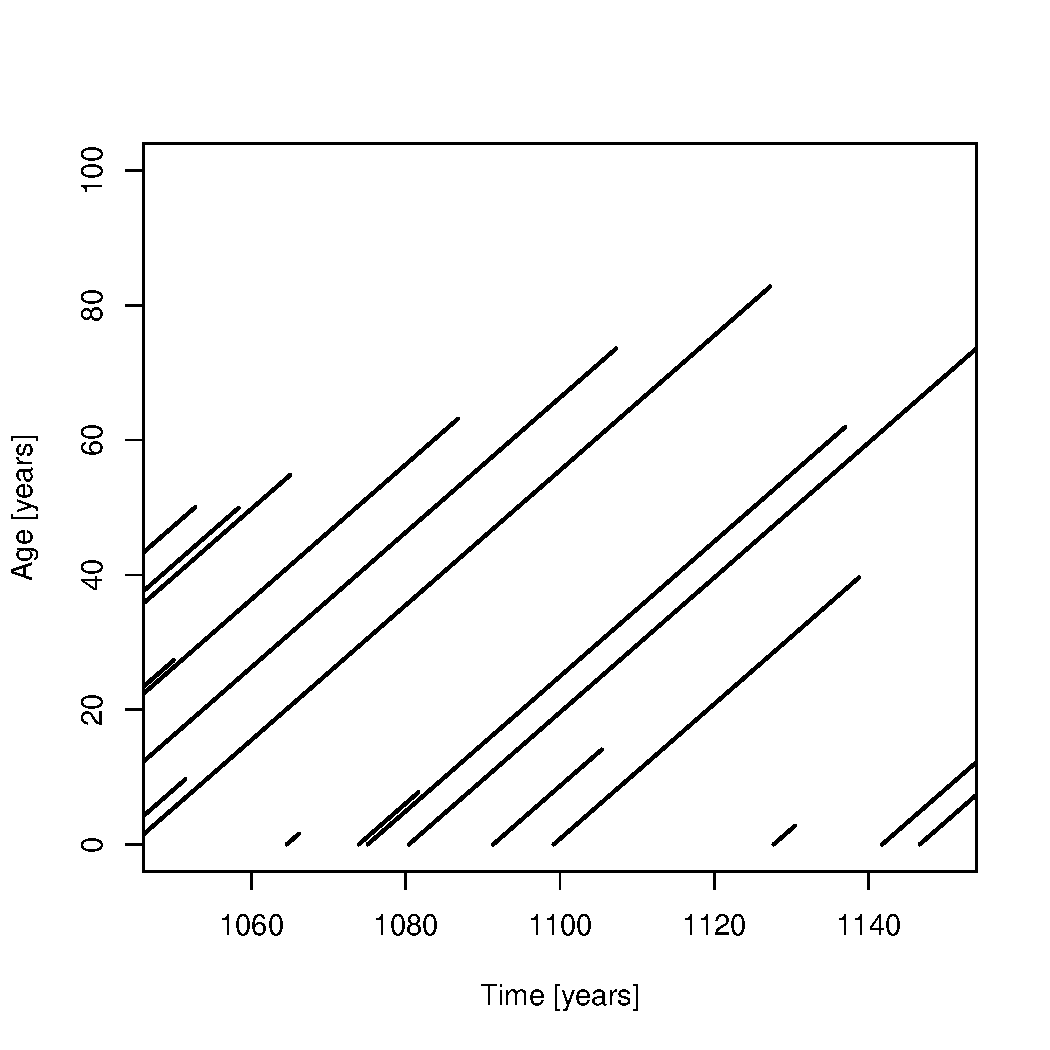
\includegraphics[height=.85\textheight]{lifeline_plot_no_horiz_line.pdf}
    \end{center}
\end{frame}

%----------- slide --------------------------------------------------%
\begin{frame}
  \frametitle{Problem Statement}
    \begin{center}
      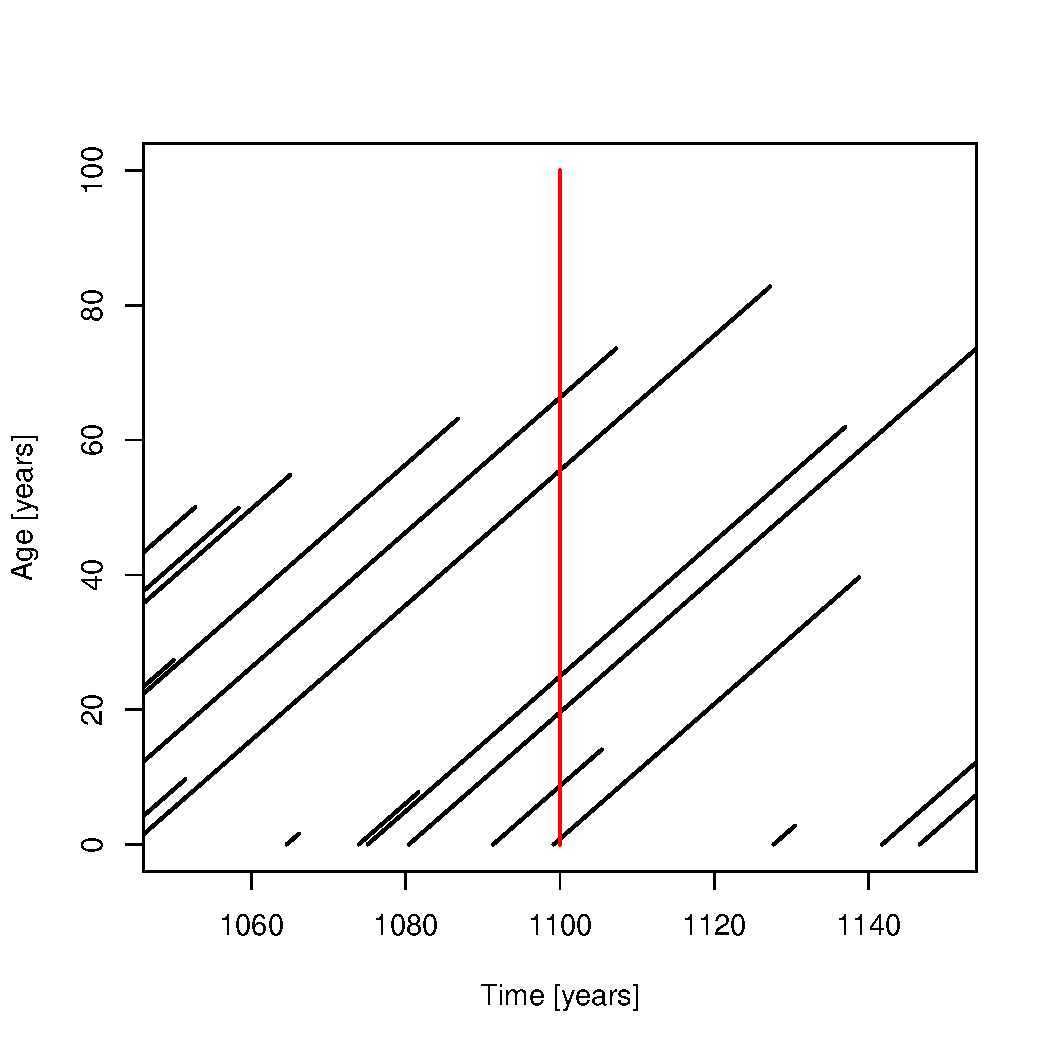
\includegraphics[height=.85\textheight]{lifeline_plot.pdf}
    \end{center}
\end{frame}

%----------- slide --------------------------------------------------%
\begin{frame}
  \frametitle{Geographic Scale}
  \begin{columns}[c]
   \column{.5\textwidth}
     \begin{block}{Site Demography}
      \begin{center}
        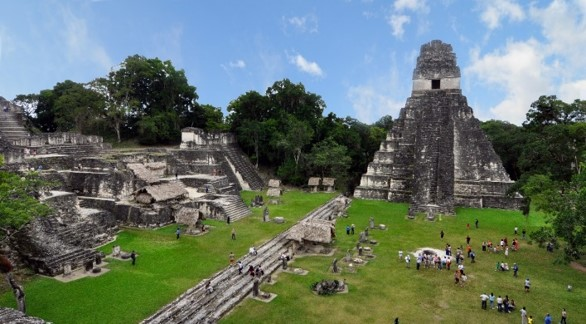
\includegraphics[width=1\textwidth]{maya_site.jpg}\
      \end{center}
    \end{block}
    \pause

   \column{.5\textwidth}
     \begin{block}{Regional Demography}
      \begin{center}
        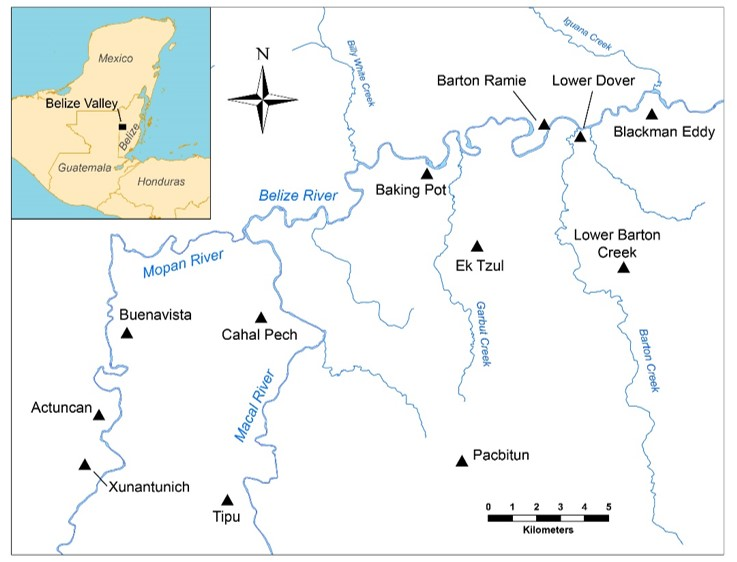
\includegraphics[width=1\textwidth]{belize_region.jpg}\
      \end{center}
    \end{block}
  \end{columns}

  \btVFill
  \small Images courtesy Julie Hoggarth \normalsize
\end{frame}

%----------- slide --------------------------------------------------%
\begin{frame}[t]
  \frametitle{Relevant Data}
  \begin{columns}[c]
   \column{.5\textwidth}
     \begin{block}{Direct}
     \begin{itemize}
       \pause
       \item{Date of Death [C14]} 
       \pause
       \item{Age at Death} 
       \pause
       \item{Isotopes} 
       \pause
       \item{DNA} 
     \end{itemize}
     \end{block}
    \pause

    \column{.5\textwidth}
     \begin{block}{Indirect}
     \begin{itemize}
       \pause
       \item{Pottery} 
       \pause
       \item{Charcoal} 
       \pause
       \item{House Counts} 
       \pause
       \item{etc.} 
     \end{itemize}
     \end{block}
  \end{columns}
\end{frame}

%----------- slide --------------------------------------------------%
\begin{frame}[t]
  \frametitle{A Tale of Two Problems: The Bias Problem}
  \pause
  \begin{itemize}
    \item A living population generates dateable material.
    \pause
    \item The amount of material is proportional to population size.
    \pause
    \item The material gets deposited in recoverable contexts.
    \pause
    \item Geological and taphonomic processes filter the material that persists to the present.
    \pause
    \item Archaeological sites are identified via survey, construction, or other means.
    \pause
    \item Archaeologists choose to excavate some of those sites.
    \pause
    \item A subset of dateable material is in fact dated.
    \pause
    \item A subset of dates are published or otherwise available for meta-analysis. 
    \pause
  \end{itemize}
\end{frame}

%----------- slide --------------------------------------------------%
\begin{frame}[t]
  \frametitle{A Tale of Two Problems: The Summary Problem}
  \pause
  \begin{itemize}
    \item Summed probability densities (SPDs) are the dominant, current method of summarizing sets of radiocarbon dates
    \pause
    \item SPDs are fundamentally flawed
    \pause
    \item A principled solution of the summary problem must be end-to-end
  \end{itemize}
\end{frame}

%----------- slide --------------------------------------------------%
\begin{frame}[t]
  \frametitle{Bayesian Inference on a Single Sample}
    \begin{center}
      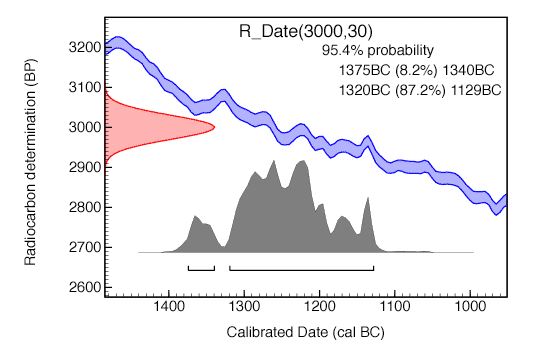
\includegraphics[height=.8\textheight]{calibration.png}
	\begin{textblock*}{100pt}(0pt,240pt)
      		\small OxCal Website \normalsize
	\end{textblock*}
    \end{center}
\end{frame}

%----------- slide --------------------------------------------------%
\begin{frame}[t]
  \frametitle{Bayesian Inference on a Single Sample: Uniform Prior}
    \begin{center}
      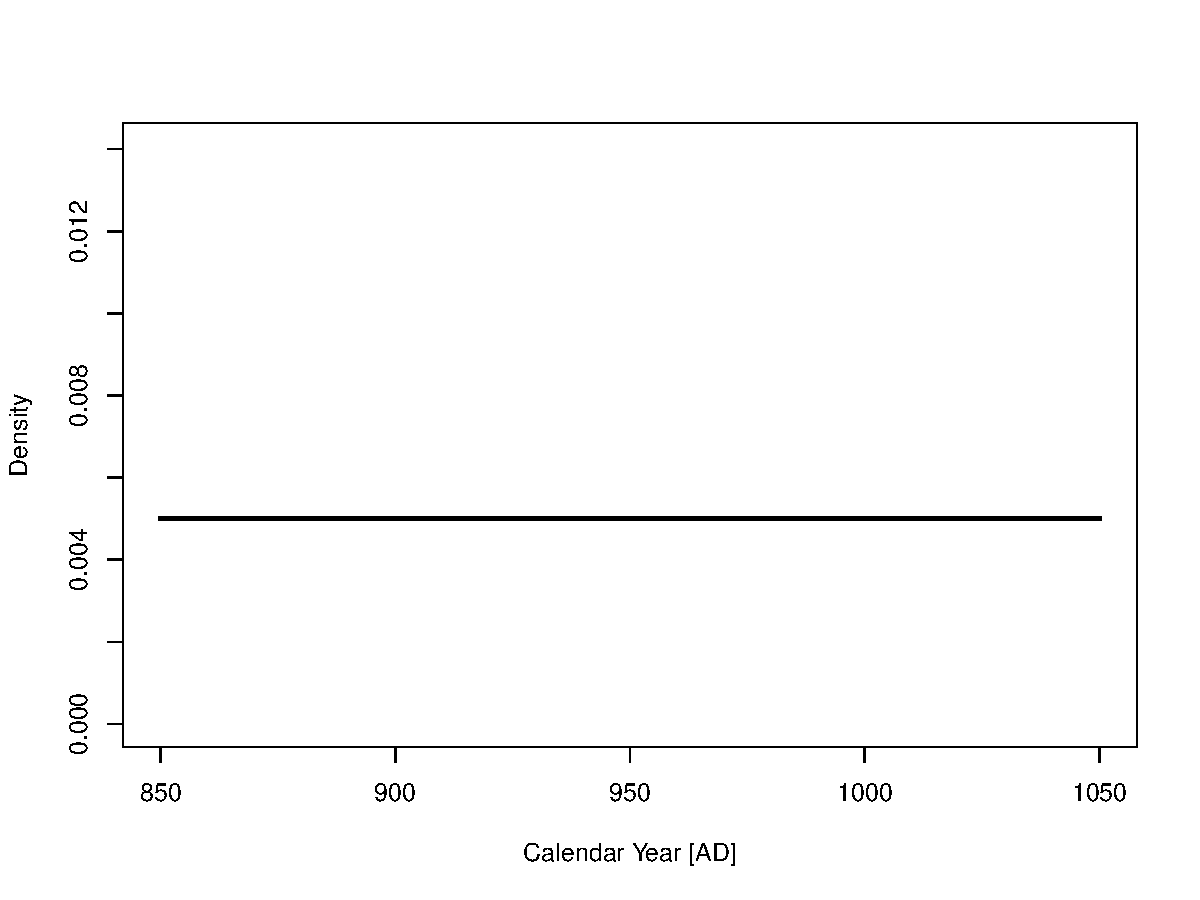
\includegraphics[height=.8\textheight]{single_obs_inf_plot1.pdf}
    \end{center}
\end{frame}

%----------- slide --------------------------------------------------%
\begin{frame}[t]
  \frametitle{Bayesian Inference on a Single Sample: Uniform Prior}
    \begin{center}
      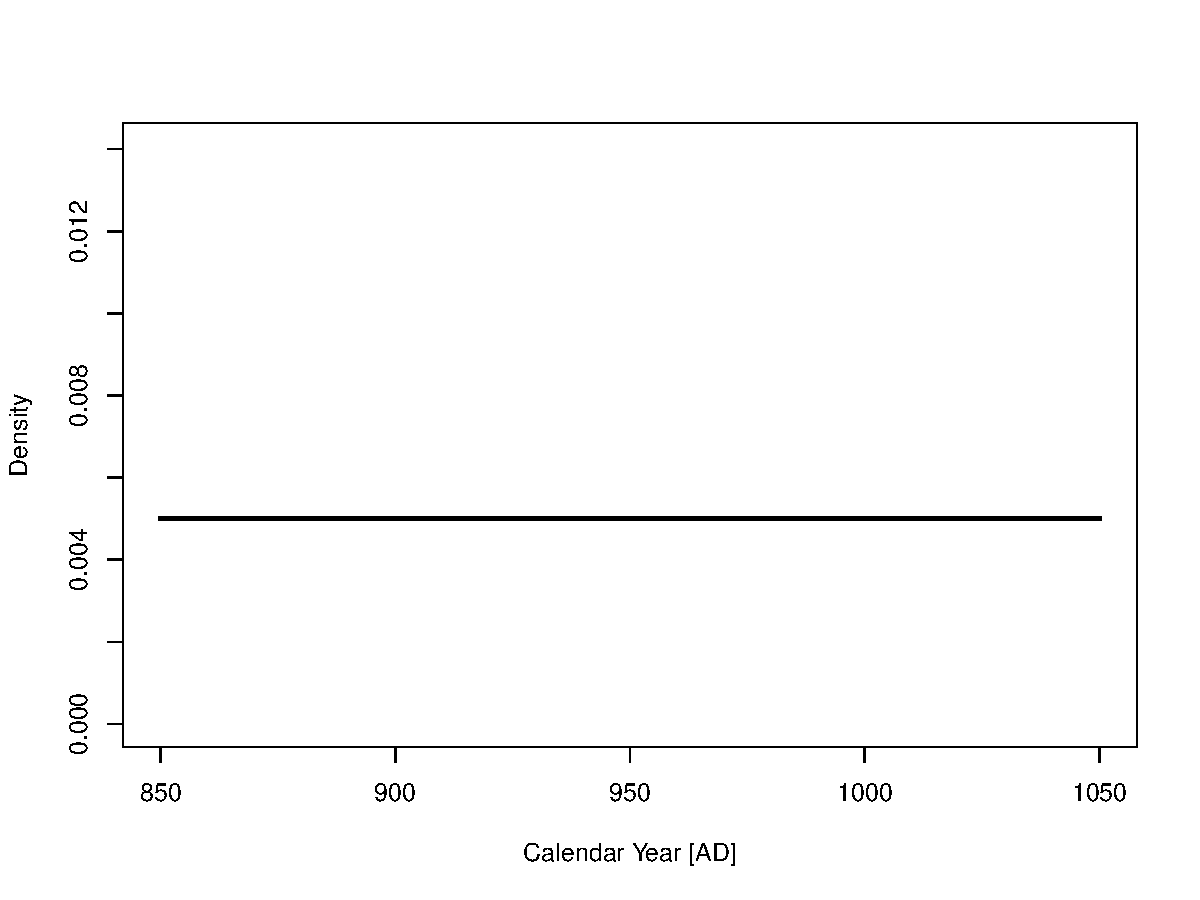
\includegraphics[height=.8\textheight]{single_obs_inf_plot1.pdf}
    \end{center}
    \begin{textblock*}{100pt}(170pt,150pt)
      \Large $p(t)$ \normalsize
	\end{textblock*}
\end{frame}

%----------- slide --------------------------------------------------%
\begin{frame}[t]
  \frametitle{Bayesian Inference on a Single Sample: Update}
    \begin{itemize}
    \item Radiocarbon determination
    \pause
    \item Uncalibrated years BP
    \item $t_{m}$
    \pause
    \item Uncertainty, uncalibrated years BP
    \item $\sigma_{t_m}$
    \pause
    \item Fraction Modern
    \item $\phi_m = \exp(-\frac{t_m}{8033})$
    \item $\sigma_m = \sigma_{t_m} \frac{\phi_m}{8033}$
    \pause
    \item
    \item Calibration curve
    \item
    \item Stratigraphy
    \end{itemize}
\end{frame}

%----------- slide --------------------------------------------------%
\begin{frame}[t]
  \frametitle{Bayesian Inference on a Single Sample: Calibration Curve}
    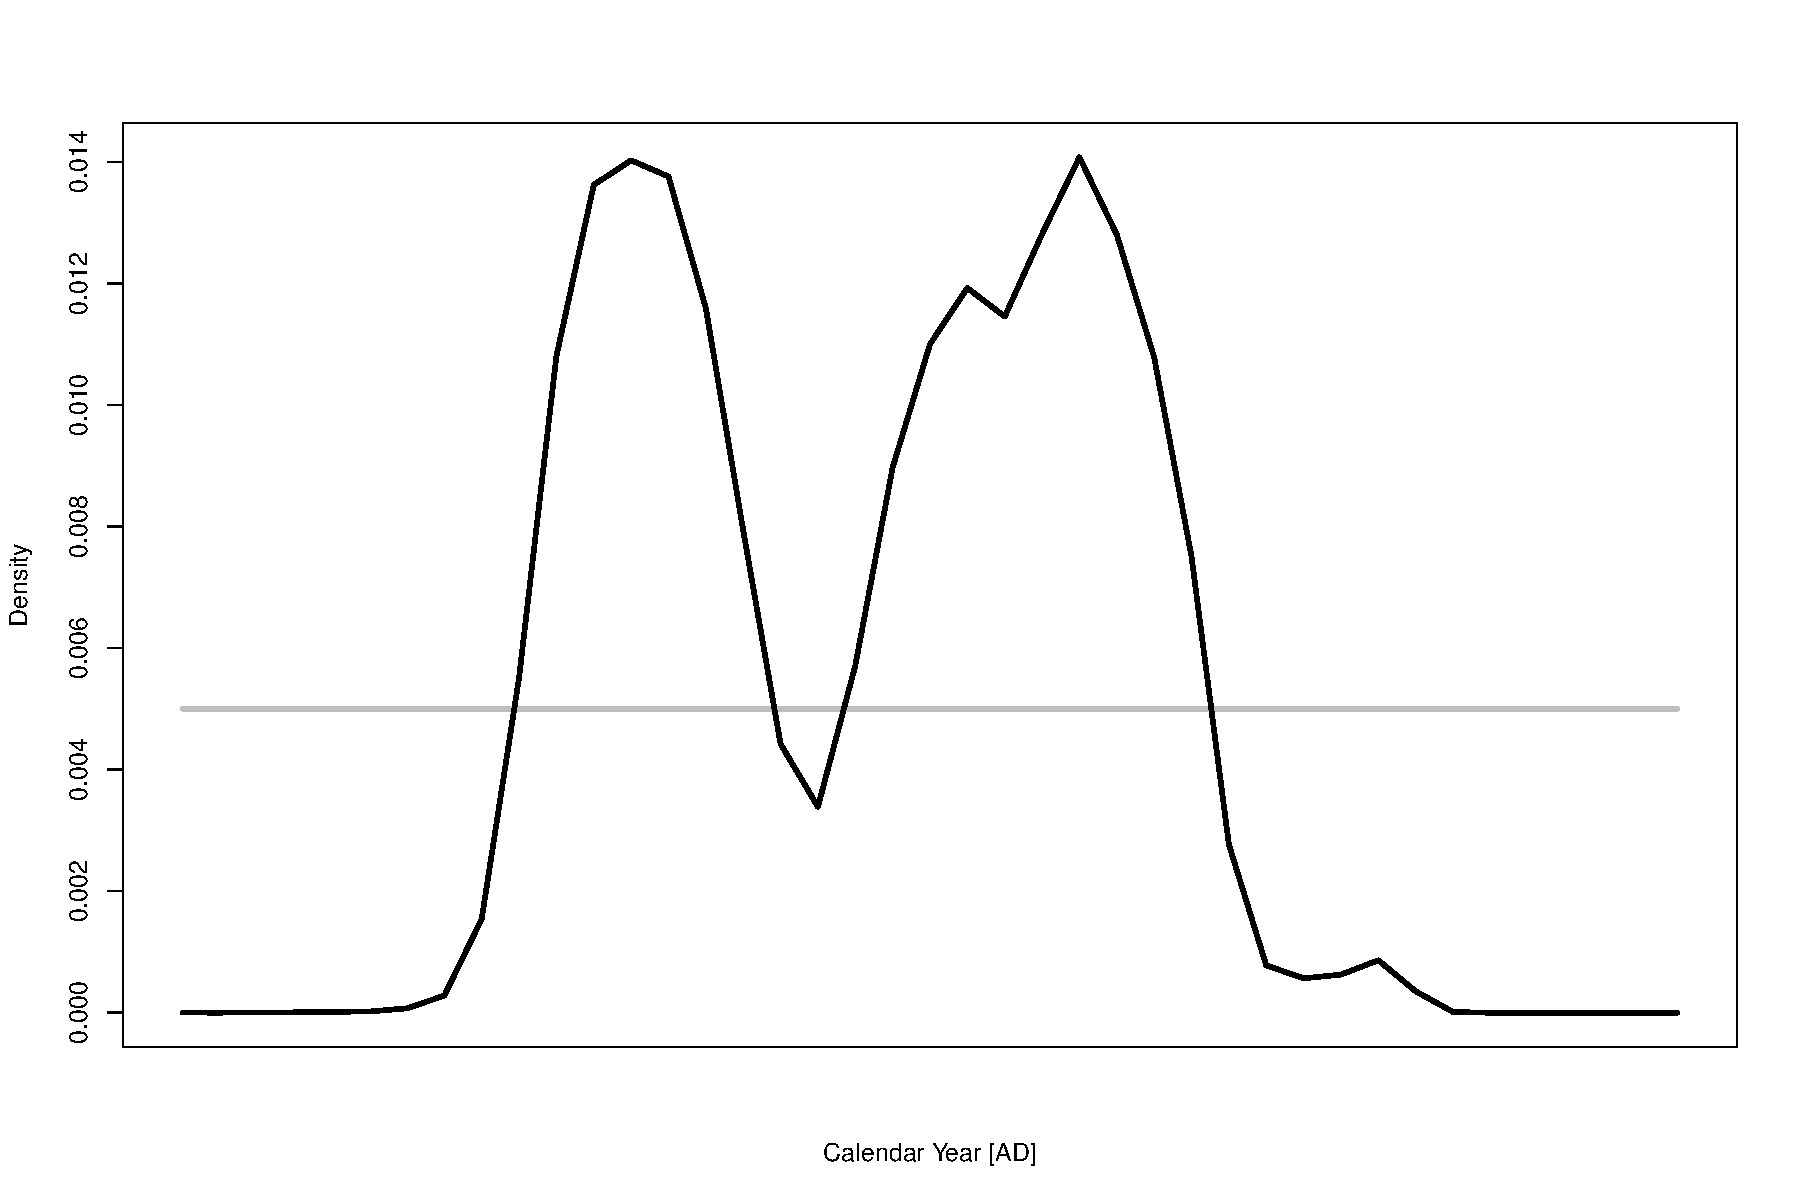
\includegraphics[height=.85\textheight]{single_obs_inf_plot2.pdf}
    
  %\begin{equation}
%  \label{eq:p_phi_given_y}
%  p(\phi_{m,i}|t) = f_{\mathcal{N}}(\phi_{m,i}|\phi_{c}(t),\sigma_i(t)) \mbox{,}
%\end{equation}

%    $\phi_m = \exp(-\frac{t_m}{8033})$
%    $\sigma_m = \sigma_{t_m} \frac{\phi_m}{8033}$
\end{frame}





\end{document}